% =====================================================================================
%  Bitacora del proyecto: identificacion automatica de particulas en Skipper-CCD
%  Documento vivo: actualizar la version, las secciones y el registro de cambios (Sec. 8)
%  a medida que avance el proyecto. Las figuras se regeneran con generar_figuras.py.
%  Compilar:  pdflatex bitacora.tex   (dos veces, para las referencias cruzadas)
% =====================================================================================
\documentclass[10pt,a4paper]{article}
\usepackage[T1]{fontenc}
\usepackage[utf8]{inputenc}
\usepackage[spanish,es-tabla,es-noshorthands]{babel}
\usepackage{lmodern}
\usepackage[margin=1.9cm,top=1.7cm,bottom=1.8cm]{geometry}
\usepackage{graphicx}
\usepackage{booktabs}
\usepackage{tabularx}
\usepackage{xcolor}
\usepackage{enumitem}
\usepackage{caption}
\usepackage{microtype}
\usepackage[colorlinks=true,linkcolor=blue!50!black,citecolor=blue!50!black,urlcolor=blue!50!black]{hyperref}

\setlist{itemsep=1pt,topsep=2pt,parsep=0pt}
\captionsetup{font=small,labelfont=bf}
\setlength{\parskip}{3pt}
\setlength{\parindent}{0pt}

\newcommand{\version}{0.8}
\newcommand{\fecha}{27 de septiembre de 2026}
\newcommand{\eminus}{e$^-$}
\newcommand{\abierto}[1]{\textcolor{orange!80!black}{\textbf{[abierto]} #1}}

\title{\vspace{-8mm}\textbf{Identificación automática de partículas en imágenes de Skipper-CCD}\\[2pt]
\large Bitácora del proyecto --- versión \version}
\author{Theo Del Compare \quad y \quad Santiago Romero \\ {\small (desarrollo asistido por Claude, Anthropic)}}
\date{\fecha}

\begin{document}
\maketitle
\vspace{-6mm}

\begin{abstract}
\noindent Se desarrolló un sistema que recibe una imagen de un Skipper-CCD, encierra cada traza en una caja y
la clasifica como \emph{muón}, \emph{electrón}, \emph{alfa}, \emph{depósito puntual} o \emph{artefacto},
con la energía depositada. Como no había etiquetas, las trazas se auto-etiquetan con reglas morfológicas
en unidades físicas, tras calibrar cada amplificador en electrones. Con esas etiquetas se entrenó un
detector YOLO11n. El sistema se ofrece como un \emph{applet} web para otros usuarios y como un kit para
reentrenarlo con datos propios. Los papers del instrumental permitieron identificar los datos (Atucha-II),
validar la calibración (ruido, masa activa, línea K del cobre) y agregar la convención de clases de CONNIE.
\end{abstract}

% -------------------------------------------------------------------------------------
\section{Datos e instrumental}
Los sensores son Skipper-CCD diseñados por LBNL y fabricados por Teledyne-DALSA, con píxeles de
$15\times15~\mu$m$^2$ y 675~$\mu$m de espesor. Promediando $N$ lecturas no destructivas por píxel se
obtiene ruido sub-electrónico~\cite{tiffenberg2017}. Se analizaron dos conjuntos (Tabla~\ref{tab:datos}).

\begin{table}[h]
\centering\small
\caption{Conjuntos de datos. Ganancia y ruido medidos en este trabajo (medias de 30 imágenes; dispersión $<1\%$).}
\label{tab:datos}
\begin{tabularx}{\textwidth}{@{}lXX@{}}
\toprule
 & \textbf{Run 43 (31/03/2025) --- Atucha-II} & \textbf{Darks (11/12/2020)} \\
\midrule
Archivos & 492 FITS, 4 amplificadores c/u & 9 FITS + 9 ROOT, 4 amplificadores \\
Geometría & CCD $6144\times1024$ px; $550\times320$ por amp., binning $\times10$ en columnas & $400\times493$ por amp., sin binning \\
Lectura & $N=300$ muestras; 53.7~min por imagen & $N=300$, exposición 600~s \\
Exposición & $\sim$32~min por píxel: imagen de limpieza entre imágenes científicas (inferido, ver texto) & 600~s \\
Orientación & CCD vertical, eje $x$ hacia arriba (\cite{depaoli2024}, Fig.~2; confirmado con los muones) & horizontal (inferido de los muones) \\
Ganancia [ADU/\eminus] & 865 / 859 / 748 / 772 & 502 / 503 / 603 / 570 \\
Ruido [\eminus] & 0.21 / 0.19 / 0.28 / 0.26 (publicado: 0.17 en 2 de 4 cuadrantes~\cite{depaoli2024}) & 0.17 / 0.17 / 0.14 / 0.15 \\
Masa activa & 2.217~g (publicado: 2.22~g~\cite{depaoli2024}) & --- \\
\bottomrule
\end{tabularx}
\end{table}

\textbf{Identificación.} La geometría ($6144\times1024$ px, $9.216\times1.536$~cm$^2$), el binning $\times10$
y $N=300$ coinciden con el Skipper-CCD instalado en la central Atucha~II, a 12~m del núcleo~\cite{depaoli2024}.
El paper informa que sólo dos cuadrantes alcanzan 0.17~\eminus: eso concuerda con lo que medimos de forma
independiente (amplificadores 0--1 nominales, 2--3 con $\sim$50\% más ruido). \abierto{El origen de los darks
de 2020 no está documentado en los papers.}

\textbf{Exposición y orientación.} El run 43 es posterior a los datos del paper. Sólo están las imágenes de
RUNID impar: cada una tarda 53.7~min en leerse y entre dos consecutivas hay 10.1~min, donde va la imagen par.
Coincide con el modo del DATA SET~B de~\cite{depaoli2024}: una lectura rápida de limpieza entre imágenes
científicas. Un píxel leído en la fracción $f$ de la imagen se limpió en la fracción $f$ de la limpieza, así que
su exposición es $10.1 + (53.7 - T_\mathrm{limp})\,f$~min: en promedio 32~min si toda la pausa es limpieza
(hasta 37~min si es más corta). \abierto{Confirmar con una imagen par (debería tener $N=1$).} El paper indica
que el conjunto está montado en vertical; en la Fig.~2 la caja del CCD cuelga con el lado largo (el eje $x$ de
la imagen) hacia arriba. Los datos lo confirman: de los muones largos del run 43, 582 forman menos de
15$^\circ$ con $x$ y sólo 12 más de 75$^\circ$. En los darks las direcciones no tienen preferencia.

% -------------------------------------------------------------------------------------
\section{Método}
\textbf{Calibración} (\texttt{particulas/core.py}). En cada amplificador:
\begin{itemize}
\item Pedestal por fila a partir del overscan; ruido estimado con la MAD del overscan.
\item Ganancia: ajuste del histograma de píxeles con un modelo gaussiano $\otimes$ Poisson (picos de 0, 1,
  2\ldots\ \eminus). Es el mismo principio que usa Atucha-II: distancia entre el pico de 0 y el de 1~\eminus~\cite{depaoli2024}.
\item Energía: $E = 3.75$~eV por par electrón-hueco.
\item Se enmascaran columnas anómalas (prescan, columnas calientes) y los NaN.
\end{itemize}

\textbf{Reconstrucción.} Umbral con histéresis: una semilla $\geq 20$~\eminus{} y crecimiento en píxeles
vecinos $\geq 4$~\eminus. Cada componente conexa es una traza. Si un cluster contiene una recta dominante
(un muón que cruza otra traza), se separa con RANSAC. La geometría se mide en píxeles \emph{físicos}
(la coordenada $x$ se multiplica por el binning), con largo, ancho transversal ponderado por carga y sagita.

\textbf{Auto-etiquetado} (Tabla~\ref{tab:reglas}). Las clases siguen la taxonomía usada en CONNIE~\cite{mirthis2025,mirthis2026}.
Los depósitos puntuales se subdividen según esa convención: \emph{blob} ($>600$~eV) y \emph{difusión}
($<600$~eV), donde caen los candidatos a CE$\nu$NS.

\begin{table}[h]
\centering\small
\caption{Reglas de clasificación (umbrales en \texttt{Params}, \texttt{particulas/core.py}).}
\label{tab:reglas}
\begin{tabular}{@{}ll@{}}
\toprule
Clase & Criterio \\
\midrule
Artefacto & línea de 1 fila (evento del registro serie, SRE) o de 1 columna (columna caliente); línea \\
 & \quad horizontal corta sin difusión vertical ($\sigma_y<0.3$~px~\cite{depaoli2024}) y sin energía de MIP \\
Alfa & $\geq 1$~MeV en una mancha compacta ($\leq 60$~px) y redonda; el núcleo satura el ADC \\
Puntual & largo $\leq 7$~px (difusión limitada): \emph{blob} si $E>600$~eV, \emph{difusión} si $E<600$~eV \\
Muón & largo $\geq 30$~px, ancho/largo $\leq 0.10$, sagita/largo $\leq 0.03$ (traza recta) \\
Muón corto & recta de 7--30~px (15--30 con binning) con la energía de una MIP que cruza los 675~$\mu$m \\
Electrón & resto: trazas curvas o irregulares (``gusanos'', Compton, beta) \\
\bottomrule
\end{tabular}
\end{table}

\textbf{Muones cortos} (v0.5). Un muón cruza todo el espesor, así que su largo proyectado es
$L = 45\tan\alpha$~px ($\alpha$: ángulo con la normal al CCD) y deposita la energía de una MIP a lo largo de
$\sqrt{(15L)^2+675^2}$~$\mu$m. El corte original ($L\geq30$~px, $\alpha\geq34^\circ$) dejaba afuera, en un CCD
horizontal, a la mitad de los muones: en los darks, las rectas cortas se clasificaban como electrones. La banda
de energía se toma de los muones largos del mismo tipo de imagen (p5 a $1.5\times$p98): 0.126--0.57~keV/$\mu$m
sin binning y 0.236--0.79 con binning. \abierto{La diferencia entre ambas escalas no está explicada.}
El criterio se validó con un Monte Carlo de flujo $\propto\cos^2\theta$ con la orientación de cada CCD y el
recorte al cuadrante (Tabla~\ref{tab:cortos}). Por debajo de 7~px (15 con binning) no se distinguen de otros
depósitos y no se reclasifican. Una prueba independiente, el gradiente de difusión a lo largo de la traza, no
sirvió: en los darks ni los muones largos lo muestran ($\sigma\approx0.4$--0.6~px).

\begin{table}[h]
\centering\small
\caption{Muones por largo proyectado: regla v0.5 / predicción del MC (normalizada con $L\geq30$~px).}
\label{tab:cortos}
\begin{tabular}{@{}lcccccc@{}}
\toprule
Largo [px] & 7--15 & 15--30 & 30--45 & 45--60 & 60--90 & $>90$ \\
\midrule
Darks (CCD horizontal) & 32 / 34 & 84 / 72 & 44 / 47 & 20 / 23 & 22 / 16 & 9 / 6 \\
Run 43, 41 imágenes (CCD vertical) & 9 / 44 & 263 / 242 & 415 / 402 & 348 / 402 & 508 / 566 & 779 / 813 \\
\bottomrule
\end{tabular}
\end{table}

\textbf{Detector.} YOLO11n (Ultralytics~\cite{yolo11}) entrenado desde pesos genéricos con las etiquetas
automáticas. Cada amplificador es una imagen de 3 canales: $\log E$, $E$ lineal de baja energía y máscara
$\geq 4$~\eminus. Se usaron 2038 imágenes de entrenamiento y 300 de validación ($\sim$103\,000 trazas),
60 épocas y batch 8, en FP32 sin \emph{mosaic}, en una GTX~1660 SUPER ($\sim$1.5~h). Durante la inferencia
se descartan cajas sin un depósito real y se usa NMS agnóstico a la clase.

\textbf{Reconstrucción + red} (v0.6). La red dejaba fragmentos en el 19\,\% de los muones largos cruzados por
otra partícula (tramos del muón como puntual, electrón o un segundo muón). Ahora las trazas salen de la
reconstrucción, que no parte muones (0 de 73) y separa lo que los cruza. La red sólo las clasifica: cada traza
toma la clase de la caja con mayor IoU ($\geq0.3$), y las reglas clasifican las que la red no ve
(5.6\,\%). También se separan las partículas que tocan un muón aunque el conjunto siga pareciendo un muón.
En validación coincide con las reglas más que la red sola en todas las clases (electrón 79$\to$86\,\%,
muón 78$\to$80\,\%, puntual 91$\to$98\,\%). Se probó antes absorber cajas sobre la recta del muón: quitaba
$\sim$9 fragmentos pero perdía $\sim$18 partículas reales, y se descartó.

\textbf{Tramos colineales} (v0.7). Los muones partidos que quedaban casi nunca venían de cruces (5 de 55), sino
de columnas enmascaradas (27) y de huecos bajo el umbral (23). Cada tramo tenía parte de la energía y los cortos
salían como electrones. Se unen tramos rectos casi paralelos, sobre la misma recta y con hueco chico
(descontando columnas enmascaradas): muones partidos 55$\to$8; en los darks, 65 ``electrones'' eran tramos de
muones. La validación de muones cortos contra el MC no cambia y la clasificación tampoco.

\textbf{Imágenes no calibradas} (PNG, JPG, TIFF, PDF). Se convierten a \emph{pseudo-electrones}:
luminancia, recorte automático de los ejes de figuras, resta de fondo y reescalado logarítmico sobre el ruido
de la propia imagen. La geometría se conserva, pero la energía no es física y no se informa.

\textbf{Archivos ROOT.} Se leen con \texttt{uproot} y se arma en memoria el FITS equivalente: formato
\texttt{skipper2root} (\texttt{skPixTree} + encabezados en \texttt{headerTree\_N}), TTree/RNTuple genérico con
ramas $x$, $y$, píxel, o histogramas TH2. En los 9 darks, ROOT y FITS dan idénticas ganancias y trazas.

% -------------------------------------------------------------------------------------
\section{Resultados}
\begin{table}[h]
\centering\small
\caption{Detector v2 (reglas v0.5) sobre 300 imágenes de validación no vistas (15\,434 trazas). Miden acuerdo
con las reglas. Última fila: el modelo v1 contra las mismas etiquetas.}
\label{tab:metricas}
\begin{tabular}{@{}lccccc@{}}
\toprule
 & Artefacto & Muón & Electrón & Puntual & Alfa \\
\midrule
mAP50 & 0.94 & 0.90 & 0.86 & 0.88 & $\sim$0 (9 casos) \\
Precisión / recall & 0.88 / 0.89 & 0.83 / 0.82 & 0.83 / 0.78 & 0.83 / 0.92 & --- \\
mAP50 del v1 & 0.79 & 0.86 & 0.80 & 0.88 & $\sim$0 \\
\bottomrule
\end{tabular}
\end{table}

\begin{figure}[t]
\centering
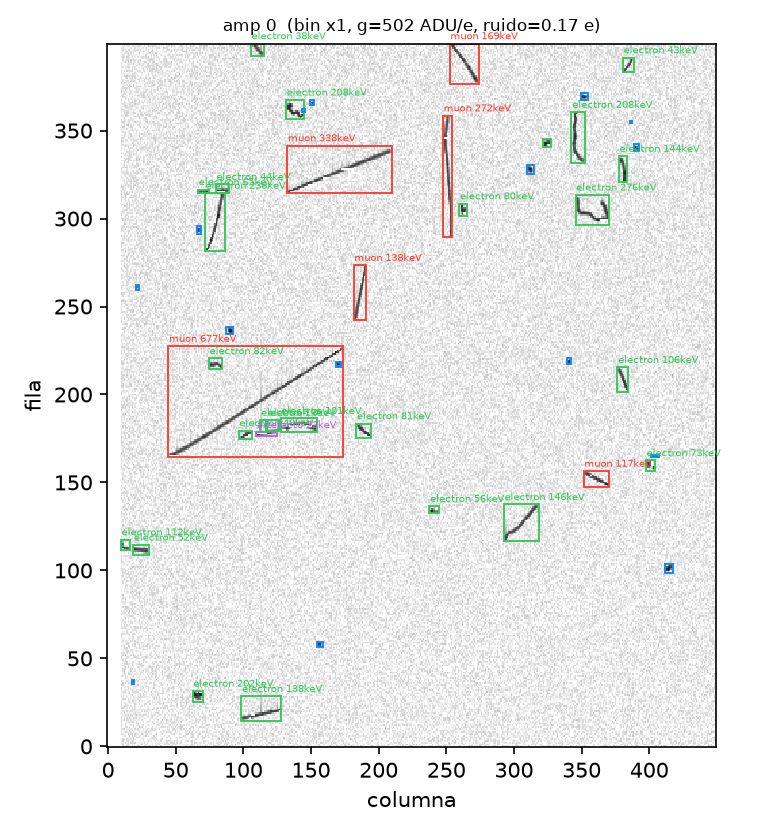
\includegraphics[width=0.49\textwidth]{figuras/detector_amp0.png}\hfill
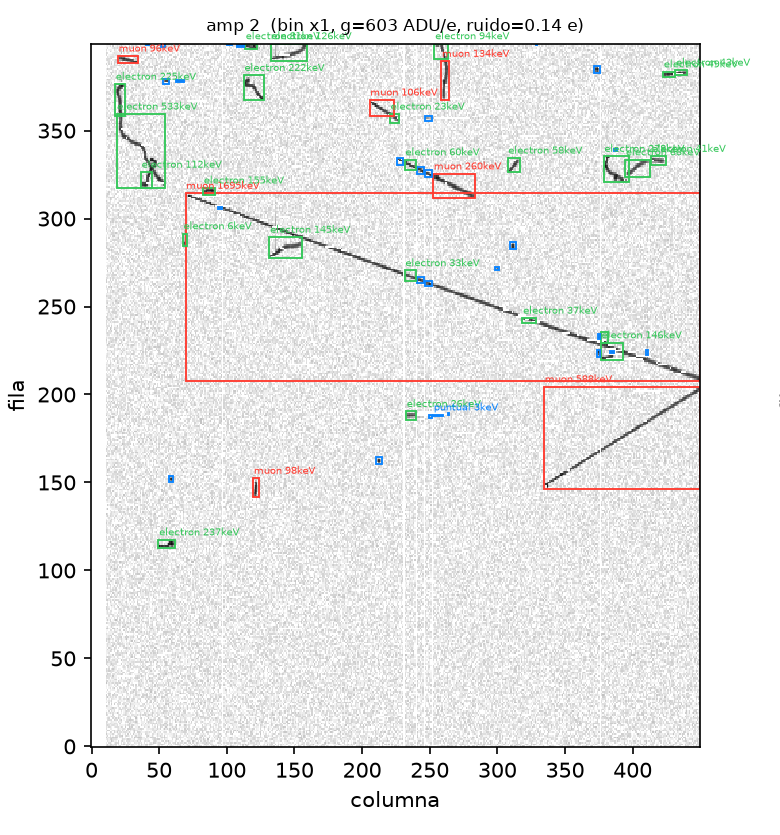
\includegraphics[width=0.49\textwidth]{figuras/detector_amp2.png}
\caption{Detecciones por reglas físicas en los amplificadores 0 y 2 de una imagen de Skipper-CCD:
muones (rojo), electrones (verde), trazas puntuales (azul) y artefactos (violeta).
Las etiquetas indican la energía reconstruida de cada traza.}
\label{fig:resultados}
\end{figure}

\textbf{Validación física con los papers.}
\begin{itemize}
\item \emph{Ruido y ganancia}: dos cuadrantes nominales y dos degradados, como informa Atucha-II~\cite{depaoli2024}.
\item \emph{Masa activa}: 2.217~g calculada con la zona activa leída, contra 2.22~g publicada.
\item \emph{Escala de energía}: aparece el pico de fluorescencia Cu~K$\alpha$ en 8~keV, la misma línea que
  Atucha-II usa para ajustar su calibración (corrección $<2\%$)~\cite{depaoli2024}.
\item \emph{Muones}: el espectro tiene su máximo en $\sim$400~keV (mediana 496~keV). Es compatible con una
  partícula de mínima ionización que cruza 675~$\mu$m de Si (0.27~keV/$\mu$m $\Rightarrow$ 180~keV en
  incidencia normal, más en trazas inclinadas).
\end{itemize}

\textbf{Detector v2 por grupo} (Tabla~\ref{tab:metricas}). De v1 a v2, la fracción llamada muón pasa del 1 al
31\,\% en los muones cortos (446), del 88 al 87\,\% en los largos y del 0.8 al 3.1\,\% en los electrones rectos
cortos. El 65\,\% de los muones cortos sigue saliendo como electrón: la red ve la energía por unidad de largo
sólo de forma indirecta. Los eventos cortos del registro serie pasan de 0 a 66\,\% reconocidos como artefacto.

\textbf{Composición típica} (Atucha-II, por imagen): 208 trazas, de las cuales 99 son electrones, 57 puntuales,
44 muones y 9 artefactos (reglas v0.4). \textbf{Tasa de muones.} Con CCD horizontal y 53.7~min de
exposición se esperaban $\sim$760 muones por imagen a nivel del mar ($\sim$1~cm$^{-2}$min$^{-1}$ sobre
14.2~cm$^2$). Un plano vertical recibe la mitad del flujo ($\pi/4$ contra $\pi/2$ para $\cos^2\theta$) y la
exposición media es $\sim$32~min, así que se esperan $\sim$230. Con las reglas v0.5 se cuentan 57 por imagen
(50 con v0.4; 41 imágenes). \abierto{Queda un factor $\sim$4. El techo de 7--17~m.w.e.~\cite{depaoli2024}
explica una parte, que no cuantificamos.}

\textbf{Imágenes no calibradas.} Sobre un amplificador con 80 trazas en el FITS:
\begin{itemize}
\item PNG gris, invertido, JPEG y PNG de 16 bits: detectan 78--79, con los mismos muones.
\item Figuras de matplotlib o PDF: detectan 49--52, por el re-muestreo de la figura.
\item Figuras con escala lineal saturada: sobrestiman los puntuales.
\end{itemize}

% -------------------------------------------------------------------------------------
\section{Herramientas desarrolladas}
El repositorio \texttt{Proyecto-detector} se organiza en dos kits sobre una librería común (\texttt{particulas/}):
\begin{itemize}
\item \textbf{\texttt{listo\_para\_usar/}} --- modelo entrenado y \emph{applet} web (Gradio). Se suben FITS, ROOT o
imágenes y devuelve:
  \begin{itemize}
  \item cada imagen con las trazas identificadas;
  \item el conteo por clase, con blobs y difusión por separado;
  \item el espectro de energía con las líneas del Cu;
  \item las tasas en eventos/(g$\cdot$día);
  \item un ZIP con PNG, CSV y FITS convertidos.
  \end{itemize}
  Además reconoce el instrumento por el encabezado (Atucha-II, CONNIE o genérico), avisa si un amplificador
  tiene más ruido que el publicado, y permite bajar el umbral a 45~eV (Atucha-II) o 15~eV (CONNIE)~\cite{connie2025}.
  En este último caso, lo que el detector no vio en el entrenamiento se completa con las reglas.
\item \textbf{\texttt{para\_entrenar/}} --- modelo sin entrenar (YOLO11n genérico) y el paso a paso:
  revisar etiquetas $\rightarrow$ construir el dataset con datos propios (FITS o imágenes) $\rightarrow$ entrenar.
\end{itemize}

% -------------------------------------------------------------------------------------
\section{Aplicaciones}
\begin{enumerate}
\item \textbf{Control de calidad en línea.} Una imagen de Atucha-II tarda 53~min en leerse y el análisis
  $\sim$5~s. Se puede seguir imagen por imagen el ruido por cuadrante, los eventos del registro serie, las
  columnas calientes y la estabilidad de la ganancia.
\item \textbf{Fondo y blindaje.} Tasas por clase (muones, electrones Compton, alfas) para comparar
  períodos reactor ON/OFF, cambios de blindaje (plomo, polipropileno) o sitios de instalación.
\item \textbf{Preselección de eventos de baja energía.} Los depósitos de difusión ($<600$~eV) contienen los
  candidatos a CE$\nu$NS y a nueva física (p.\,ej.\ partículas milicargadas~\cite{connie2025}). Clasificar las
  trazas grandes permite vetarlas y estudiar su contaminación en la región de interés.
\item \textbf{Pre-etiquetado para anotación manual.} CONNIE anotó a mano $\sim$4200 eventos con una GUI de
  anotación redundante~\cite{mirthis2026}. Las etiquetas sugeridas por el detector pueden acelerar ese trabajo,
  y ese dataset, a su vez, puede reentrenar el detector.
\item \textbf{Verificación de calibración y exposición.} Con la línea Cu~K$\alpha$ y la masa activa se chequea
  la escala de energía y la normalización de cada \emph{run}.
\item \textbf{Contaminación radiactiva.} Las alfas son raras y suelen indicar contaminación externa~\cite{mirthis2025}:
  su tasa sirve para monitorear materiales.
\item \textbf{Otros experimentos y docencia.} El kit de entrenamiento permite adaptar el sistema a otros
  Skipper-CCD (SENSEI, DAMIC-M, Oscura). La lectura de PNG/PDF permite usarlo con imágenes publicadas o en
  actividades de divulgación.
\end{enumerate}

% -------------------------------------------------------------------------------------
\section{Limitaciones y trabajo futuro}
\begin{itemize}
\item \textbf{Etiquetas automáticas.} Las métricas miden el acuerdo con las reglas, no con la partícula
  real. Próximo paso: reentrenar con el dataset anotado de CONNIE, donde DenseNet-121 con estrategia
  uno-contra-todos alcanza 0.93 de exactitud~\cite{mirthis2026}, o con simulaciones Geant4.
\item \textbf{Alfas.} Sólo 45 en todo el dataset. Hay que sumar datos o simulaciones.
\item \textbf{Trazas cruzadas.} Hace falta una clase ``otros'' para trazas cruzadas, como en CONNIE, y
  cortes geométricos de baja energía como los de Atucha-II ($0.3<\sigma_y<1$ px)~\cite{depaoli2024}.
\item \textbf{Darks de 2020.} Tienen pocas imágenes sin binning, así que el método automático usa las reglas.
\item \textbf{Formatos.} Las imágenes ROOT ya se leen; faltan los catálogos de eventos ROOT de CONNIE (clusters
  ya reconstruidos) y corregir el \emph{cross-talk} entre cuadrantes.
\item \textbf{Muones cortos en el detector.} El v2 reconoce el 31\,\% de los que marcan las reglas. Opciones:
  revisar con la regla de energía las cajas ``electrón'' cortas del detector, o entrenar con simulaciones
  Geant4 (generador CRY) con la orientación y el binning de cada CCD, donde se conoce la partícula real.
  Se probó sumar las trazas de los darks binneadas $\times10$ sobre fondos reales de Atucha, pero se descartó:
  por la diferencia de escala de energía casi no quedan muones cortos, y las imágenes son mucho más densas.
\item \abierto{Tasa de muones: queda un factor $\sim$4 (Sec.~3). Falta confirmar la exposición con una imagen par
  y cuantificar el techo de 7--17~m.w.e.}
\end{itemize}

% -------------------------------------------------------------------------------------
\section{Registro de cambios}
% Agregar una fila por cada avance (fecha, version, que cambio). No es un flotante: queda en su lugar.
{\small\noindent
\begin{tabularx}{\textwidth}{@{}lX@{}}
\toprule
Fecha & Cambio \\
\midrule
19/09/2026 & Recepción de los datos: darks 2020 (FITS+ROOT) y run 43 (492 FITS). \\
26/09/2026 & v0.1: visor; calibración ADU$\to$\eminus; reconstrucción y reglas; dataset de $\sim$103k trazas;
  YOLO11n entrenado; \emph{applet} web con conteo y ZIP. \\
26/09/2026 & v0.2: entrada PNG/JPG/TIFF/PDF (pseudo-electrones, recorte de ejes); conversor a FITS;
  reorganización en kits \texttt{listo\_para\_usar} / \texttt{para\_entrenar}; repositorio git. \\
26/09/2026 & v0.3: lectura de papers~\cite{depaoli2024,connie2025,mirthis2025,mirthis2026}; identificación de
  Atucha-II; perfiles de instrumento; blob/difusión; espectro con líneas del Cu; tasas por masa; umbral
  configurable (225/45/15~eV); corrección de la masa activa (overscan vertical); esta bitácora. \\
27/09/2026 & v0.4: entrada ROOT en el \emph{applet} y la línea de comandos (\texttt{skipper2root}, TTree/RNTuple
  genérico, TH2), con resultados idénticos al FITS en los 9 darks; conversor ROOT$\to$FITS; licencia MIT. \\
27/09/2026 & v0.5: orientación (vertical) y exposición ($\sim$32~min) de Atucha-II a partir de~\cite{depaoli2024} y
  los datos; muones cortos validados con MC $\cos^2\theta$; SRE por $\sigma_y$; detector v2 reentrenado. \\
27/09/2026 & v0.6: las trazas salen de la reconstrucción y la red las clasifica (los muones cruzados ya no se
  parten); las reglas separan partículas pegadas a muones. \\
27/09/2026 & v0.7: unión de tramos colineales de una misma traza (columnas enmascaradas, huecos, cruces). \\
27/09/2026 & v0.8: applet abre el navegador cuando está listo (antes: conexión rechazada) y carga el modelo en
  segundo plano; kit de entrenamiento todo en uno (\texttt{mis\_datos} $\to$ modelo $\to$ applet propio) con
  criterios editables en \texttt{criterios.yaml}. \\
\bottomrule
\end{tabularx}}

\vspace{-3mm}
{\small
\begin{thebibliography}{9}\setlength{\itemsep}{0pt}
\bibitem{depaoli2024} E.~Depaoli \emph{et al.}, \emph{Deployment and performance of a Low-Energy-Threshold
  Skipper-CCD inside a nuclear reactor}, JHEP \textbf{10} (2024) 155.
\bibitem{connie2025} CONNIE y Atucha-II Collaborations, \emph{Search for Reactor-Produced Millicharged
  Particles with Skipper-CCDs at the CONNIE and Atucha-II Experiments}, PRL \textbf{134} (2025) 071801.
\bibitem{mirthis2025} S.~Mirthis, I.~Nasteva, P.~D.~P.~Costa, \emph{Particle Tracking Classification in the
  CONNIE Experiment}, ENIAC (2025).
\bibitem{mirthis2026} S.~Mirthis, \emph{Event Classification and Annotated Dataset in CONNIE}, ICHEP (2026).
\bibitem{tiffenberg2017} J.~Tiffenberg \emph{et al.}, \emph{Single-Electron and Single-Photon Sensitivity with
  a Silicon Skipper CCD}, PRL \textbf{119} (2017) 131802.
\bibitem{yolo11} G.~Jocher, J.~Qiu, \emph{Ultralytics YOLO11} (2024), \url{https://github.com/ultralytics/ultralytics}.
\end{thebibliography}}

\end{document}
